\documentclass[11pt,letter,oneside]{article}
\usepackage{sectsty,setspace} 
\usepackage[top=1.00in, bottom=1.0in, left=1in, right=1in]{geometry} 
\usepackage{graphicx}
\usepackage{epstopdf}
\usepackage{amsmath,latexsym,amssymb,wasysym}
\usepackage[english]{babel}
\usepackage{cite}
\usepackage{citesupernumber}
%\usepackage{citecollapse}
\usepackage{wrapfig}
\usepackage{hyperref}
\usepackage{float}
\restylefloat{table}
\usepackage[table]{xcolor} % http://ctan.org/pkg/xcolor
\usepackage{gensymb} % You have to have this to use \degree
\usepackage{wrapfig}
\usepackage[font=small,labelfont=bf]{caption}

\usepackage{cite}
\usepackage{citesupernumber}

\setlength\parindent{0pt} % no indents throughout

\setlength{\abovecaptionskip}{1pt}
\setlength{\belowcaptionskip}{-10pt}
\usepackage[font={small}]{caption}

\parskip=6pt
\pagenumbering{arabic}
\pagestyle{plain}
% squeeze spacey
\linespread{0.99}
\addtolength{\itemsep}{-0.05in}
\usepackage{multicol}
 
\newenvironment{smitemize}{
\begin{itemize}
  \setlength{\itemsep}{1pt}
  \setlength{\parskip}{0pt}
  \setlength{\parsep}{0pt}}
{\end{itemize}
}

\usepackage{fancyhdr}
\pagestyle{fancy}
\fancyhead[LO]{Fulbright 2026}
\fancyhead[RO]{E. M. Wolkovich}

\newcommand{\Section}[1]{\vspace{-8pt}\section{\hskip -1em.~~#1}\vspace{-3pt}} 


\begin{document}
\bibliographystyle{/Users/Lizzie/Documents/EndnoteRelated/Bibtex/styles/ajhg}
\renewcommand{\refname}{\CHead{}}

\begin{centering}
{\bf Designing climate-resilient agriculture through crop portfolios}\\ % Developing climate resilient agriculture through heat tolerant crops and their cultivars
\end{centering}
\vspace{2ex}

% TO DO. ... 
% maybe skim what is supposed to be in each section?
% Try to add a little more on why I am so perfect for this... 
% Re-read

\emph{Extended abstract:} Hotter, drier summers and increasing extremes are challenging growers across the world. This is especially clear in Europe where summer heat is increasing faster than in the Arctic. Maintaining agricultural regions that continue to provide economic livelihoods and high-quality products while continuing traditional practices requires understanding of the climate resiliency of current crops, and how to best exploit it. Here I propose to address this by leveraging new data on plant responses to heat extremes and cutting-edge genetics research in Montpellier with my skills in hierarchical modeling. Working with data across varieties and clones of one of the world's most economically important crops---winegrapes---we will quantify heat tolerance across cultivars (varieties) and clones to help growers develop climate-smart portfolios. % with extensions well beyond winegrapes 

% Shorter ... 41 characters remaining
% Hotter, drier summers and increasing extremes are challenging growers across the world. This is especially clear in Europe where summer heat is increasing faster than in the Arctic. Maintaining agricultural regions requires understanding of the climate resiliency of current crops, and how to best exploit it. Here I propose to leverage the deep agriculture knowledge, data and cutting-edge research in Montpellier with my skills in hierarchical modeling to address this. Working with unparalleled data across varieties and clones of one major crop, we will quantify heat tolerance across cultivars and clones to help growers develop climate-smart portfolios.

% This document addresses key elements of your project: what the project is, why it is needed, the objective(s) of the project, how you are prepared for the project and how you will accomplish it, the project timeline, and the outcomes and impact
% https://fulbrightscholars.org/us-scholar-awards#steps --> Project statement
% 3-5 pages
% Single-spaced, 12-point font, 1-inch margins. This helps ensure readability.
% Use headers and/or bullets to organize and convey key elements; use page numbers.
% Citations are not required in the Project Statement. You may use endnotes or footnotes in 10-point font (use any format for citations). If you are applying for Research or Teaching/Research, you may put the full citation for a source mentioned in your Project Statement in the Reference List/Bibliography.

{\bf Background}

Resilient agricultural systems today must deal with the increasing stressors of climate change.\cite{benitez2023enhancing,foley2011solutions} Hotter, drier summers and increasing extremes in heat, cold and precipitation are challenging growers across the world.\cite{ipcc2021} This is especially true in Europe where summer heat is increasing faster than anywhere else on earth.\cite{schumacher2024exacerbated} Across Europe, the Mediterranean region has emerged as one of the most impacted by increasing temperatures, with increasing reports of crop damage and failures alongside the heat.\cite{oltmanns2024,tuel2020mediterranean} 

High temperatures can slow plant development and cause tissue damage,\cite{coupel2024clusters} leading to yield declines and making it harder for growers to maintain croplands. 
% Maintaining agricultural regions that continue to provide economic livelihoods and high-quality products while continuing traditional practices relies on a greater understanding of the climate resiliency of current crops, and how to best exploit it as the climate continues to shift. 
How to develop agricultural regions that continue to provide economic livelihoods and high-quality products while continuing traditional practices with climate change is one of the greatest challenges of the next century. Meeting this challenge requires a greater understanding of the climate resiliency of current crops, and how to best exploit it as the climate continues to shift.  % Models of future food security include this reality that growers will need to shift their crops over time with increasing climate change, but how best to do this remains a major open question.

% More on the importance of heat tolerance and heat tolerance across crops and cultivars.
One of the most effective methods for climate resiliency is to exploit the diversity of existing heat tolerance in current crops.\cite{labeyrie2021role,van2019crop} Different crop species and cultivars (or varieties---meaning different plants within a crop species) require and can tolerate different levels of heat.\cite{cooper2021,wahid2007} Matching this diversity to future climates can thus allow growers to maintain many of their traditional practices and plant the same species well into the future\cite{Wolkovich2017}---depending on the climate diversity of that crop species, and how well we can estimate it. 

% Accurate forecasts of when growers should change their planting regimes with climate change require 
% Yet what temperature is too high depends on a suite of factors, but especially on the exact crop and cultivar. 
Progress in forecasting when growers should change their planting regimes with climate change has been slow because of our limited knowledge of the temperature response of different crops\cite{wang2017}. Fundamental temperature response curves (Fig. \ref{fig:tempcurve}) underlie the biology of all organisms and are critical to forecasting crops with climate change.\cite{Bennett2021,buckley2021evolution} These models usually capture the non-linear effect of temperature,\cite{parent2012} where increasing temperatures beyond some fundamental minimum (below which cells cannot grow) generally accelerate development and growth until some maximum rate---which defines the optimal temperature. Higher optima generally means higher heat tolerance---and plants that can continue to grow through some level of heat waves. At temperatures higher than this optimum, development and growth slows and then stalls, driving crop failures.\cite{luo2011temperature,anandhi2017developing}

% Then more on why we do not have good information on this to help growers adapt: the current hurdles this project will overcome. 
% Many models simply set the upper limit for many plant events at 40$\degree$C, even though this limit varies across species, populations and phenological events\cite{parent2012}.
Estimating temperature responses curves---and their critical values of the temperature minimum, optimum and maximum---is extremely difficult.\cite{garcia2010curvilinear,moralescastilla} To date most estimates of complete temperature response curves exist for only a handful of herbaceous crops that are amenable to small-scale experiments (generally done in controlled environment chambers where temperatures are held constant and rates can be carefully measured). Heat tolerance estimates in many species, and effectively all woody species, rely on modeling approaches that cannot robustly estimate temperature maxima or minima (and thus they are usually fixed) and where estimates are easily biased by data quality issues (e.g., far more data for one species than another).\cite{moralescastilla,Yang2024}

\begin{wrapfigure}{r}{0.67\textwidth}
\centering
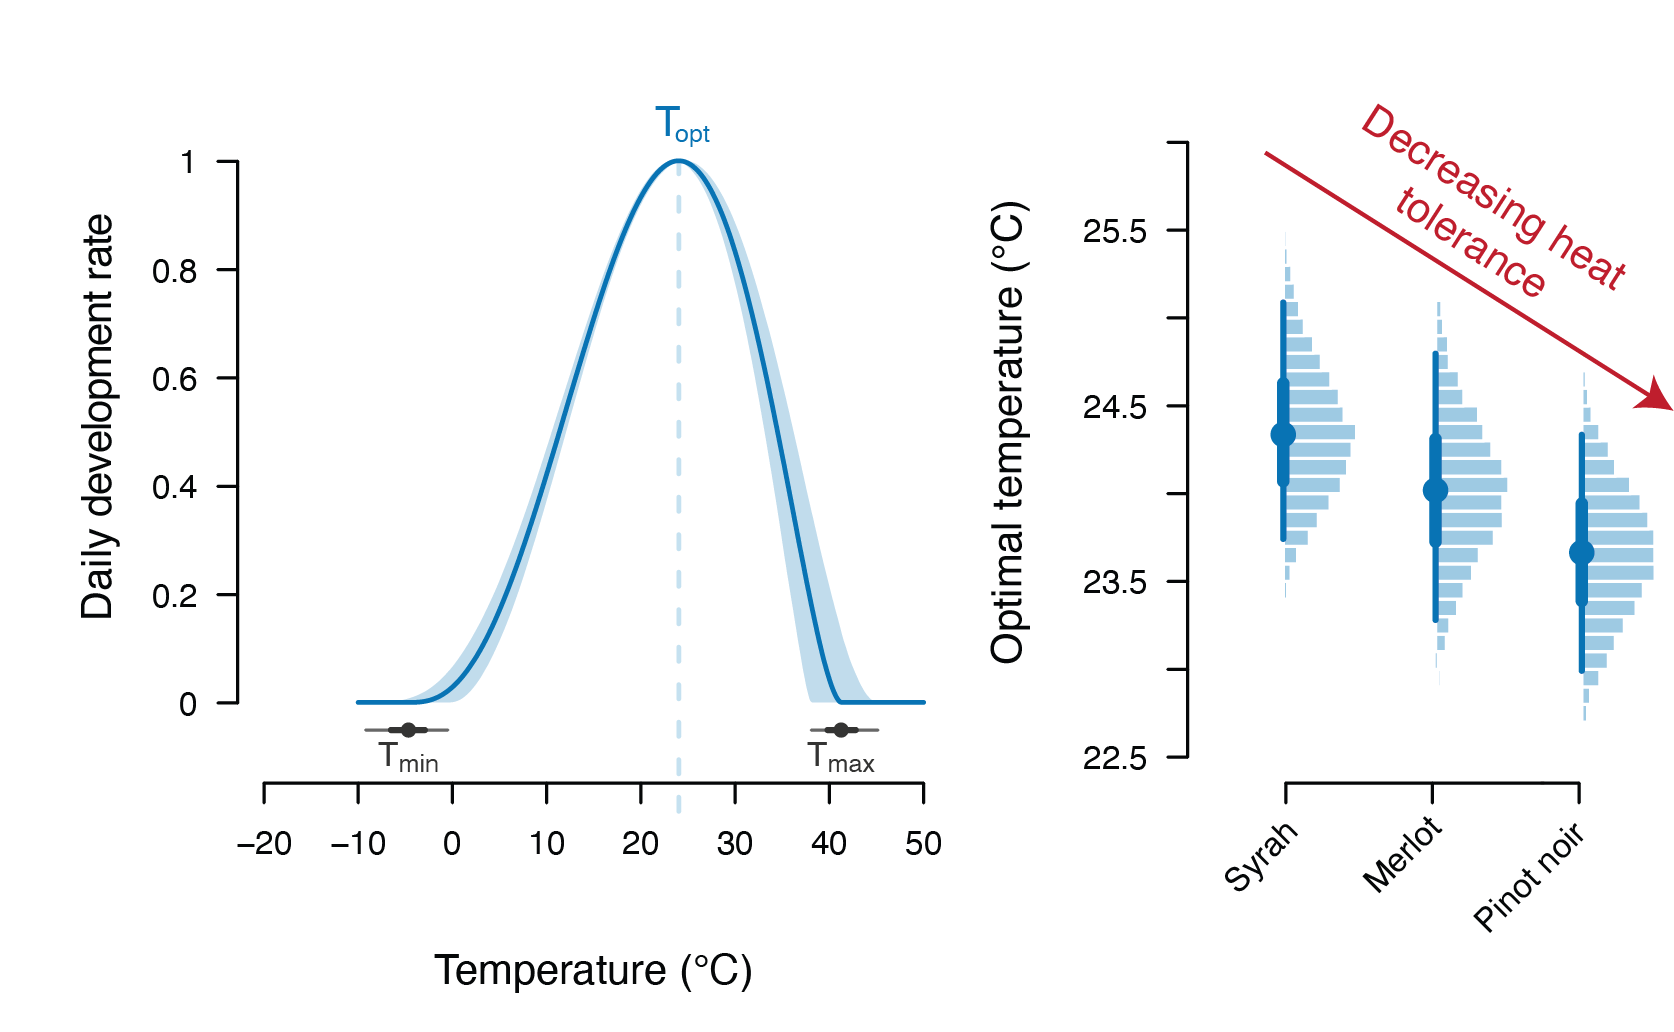
\includegraphics[width=0.65\textwidth]{figs/tempcurve_3vars_annotate.png}
\caption{This project will estimate a temperature response curve for winegrapes as a crop, including heat tolerance variation across cultivars. Response curves, as shown here, estimate the daily rate of development (or growth) from some minimum (at 0) to a daily maximum (at 1) depending on different mean temperatures. Here we show current results for veraison (left) and variation in the optimal temperature for three cultivars (right) but this project will extend to up to hundreds of different varieties and more accurately model them given genetic information.} 
\label{fig:tempcurve}
\end{wrapfigure}
\setlength{\intextsep}{6pt} 
Today, many models of future food security assume that growers will need to shift their crops over time with increasing climate change. However, they can usually only forecast major shifts---for example, from winegrapes to avocados---that would require immense human adaptation and the likely loss of traditional practices. Improved estimates of the temperature response of different crop species and their cultivars could rapidly help growers develop more climate resilient systems. Such information would allow growers to exploit the full climate diversity of their existing crop species, before considering a major shift. % Given the apparent diversity of heat tolerance within many crops, many growers may not need to switch species, depending on the crop and scale of climate change. 

Estimates across a large number of cultivars would also help growers develop climate resilient portfolios---selecting the best mix of cultivars for each grower given their preferences and region.\cite{dempewolf2014adapting,van2019crop,labeyrie2021role} A portfolio of cultivars can better handle climate variation year to year, as several may perform best in slightly cooler years and several others in slightly warmer years. At the same time, adjusting the mixture over time can help adapt to long-term trends due to anthropogenic climate change.  While the concept of a careful portfolio of climatically matched cultivars could clearly help agricultural systems, how much such portfolios are used depends on local practices and the particular crop. It also depends on growers having the information they need on how different cultivars respond to climate.\cite{van2019crop}

{\bf What?}

Working with colleagues in Montpellier, I will leverage new methods alongside newly available genetic and development data to estimate the climate resiliency of one of the world's most economically important crops\cite{faostat}---winegrapes. We plan to use winegrapes as a case study because they are important economically and culturally, and span a wide climatic gradient.\cite{ollat2023moving} Perhaps not surprisingly then, they are also highly impacted by climate change.\cite{Leeuwen2024} They also have the data on seasonal development and genetic information required to build the most robust models. While we will focus on winegrapes, our approach is specifically designed to extend to other crops. 

We plan to overcome the major data quality issues that have stymied previous efforts to estimate full temperature response curves across cultivars---called varieties in winegrapes (where each is a unique genotype)---through multi-level (also known as hierarchical) modeling.\cite{gelmanhill,BDA} This approach estimates at once an overall species-level temperature response curve at the same time it estimates differences across varieties, while accounting for uneven sampling and spatial variation. Highly uneven data across cultivars is a common problem in crops, including winegrapes, because a few varieties are often very popular, widely planted and have extensive data (e.g., Chardonnay, Pinot noir), while other varieties are less common but may harbor excellent heat tolerance or other temperature response attributes that could be make them ideal for adapting to climate change (e.g., Xinomavro).\cite{Wolkovich2017} I have developed new modeling approaches\cite{morales2024phylogenetic} that can handle this uneven sampling by incorporating genetic relatedness information on cultivars to better estimate each variety. They also can be adapted to include additional layers of genetic information. For example, within each winegrape variety multiple clones exist (where each clone has unique somatic mutation differences) and this can be further incorporated into the models to better understand climate resiliency within each variety and clone, allowing growers to fine-tune their portfolios. 

This approach relies on the extensive data and expertise of my colleagues in Montpellier, who have recently helped lead a major new analysis of the genetic relatedness of winegrape varieties, which we leverage here. They also provide a depth of knowledge of traditional practices and current challenges for winegrowing in France, making the proposed work well positioned to directly aid growers. Additionally, they have the seasonal development data required to estimate temperature response curves (described further below) observed over high temperatures. 

The lack of observational data at high temperatures has limited previous work to estimate optimum and maximum temperatures for crops, but recent heat extremes in Montpellier have pushed plants into these regions. My colleagues have been on the forefront of documenting this\cite{coupel2024clusters} and provide rare data and expertise we will leverage.  % Now is the time! We also have the extreme heat we need. 
This project thus brings together my modeling expertise, with the expertise on winegrape genetic diversity, response to heat extremes and critical regional and larger-scale understanding of winegrowing. %  human adaptation. 

{\bf How? }
%  How will you accomplish the project? Be as specific as possible regarding all aspects of your plans, including anticipated activities, methodology, required resources, and your proposed timeline. Address how you will adjust your plans if needed, including the feasibility of the project given the resources and time allocated. How is your project innovative?
% How are you prepared to carry out your project? Describe your relevant experience and how it prepares you to conduct the project (this should complement your essays and CV/Resume).
% How will you engage with the host institution/ organization and community? If applicable, address any communication you may have had with the potential host institution(s).

% Working with colleagues in Montpellier, I will develop temperature response curves for hundreds of cultivars (varieties) and clones. 
Our approach centers around (1) the domestication of winegrapes across Europe's extensive climate gradient that led to cultivars (varieties) that likely vary strongly in their heat tolerance and (2) the shared evolutionary history of winegrape cultivars that we can use for more robust estimates across diverse varieties. We will accomplish this with models that use long-term observations of seasonal development data (also called phenological data), which captures the progression of the timing of major developmental stages, from budburst to flowering, and fruit ripening (veraison). For this we will mainly leverage an incredible collection of data across hundreds of varieties, which is unique in the world for its diversity of varieties---the Vassal-Montpellier Grapevine Biological Resources Center. Alongside these data, we expect to include additional data from resources across INRAE and other regional programs that have collected data on seasonal development. Climate data will be drawn from a widely-used and validated gridded historical dataset (E-OBS),\cite{cornes2018ensemble} as well as potentially finer-scale data provided by collaborators. If time allows we will generate forecasts of the future variety suitability for European winegrowing regions using scenarios from CMIP6 (global models of future climate)\cite{eyring2016,riahiSSP2017,cookcmip} and shapefiles for winegrowing regions provided by my collaborator, Dr. Ignacio Morales-Castilla).

% I plan to leverage my existing expertise in development models, data synthesis, hierarchical Bayesian approaches\cite{flynn2018,ospreebbms} 
My collaborators in Montpellier have extensive expertise in winegrape variety diversity, viticultural practices, impacts of climate change on viticulture and how to develop more sustainable agriculture to promote biodiversity, healthy environments and food security. In preparing this application, I have worked closely with my proposed hosts Drs. Thierry Lacombe, Vincent Segura and Patrice This (who each work across varying institutes in Montpellier, including L'Institut Agro Montpellier, INRAE, UMR Agap) and plan to be formally hosted by DAAV team (Diversité, Adaptation et Amélioration de la Vigne) at the AGAP Institute (see letter by Claire Billot, director of AGAP Institute), which has a major focus on the theme of my work: adapting agriculture to climate change. My hosts are experts on variety diversity in winegrapes, especially Lacombe and This who are global leaders in the genetic diversity of winegrapes.\cite{lacombe2013large,this2006historical} They are also the scientific co-directors of Vassal-Montpellier Grapevine Biological Resources Center, where much of the data will come from. Segura provides expertise in genomic approaches including cutting-edge approaches to linking plant traits to their genetics,\cite{korte2012mixed,segura2012efficient} which will aid the project. Together, they will help select varieties for the model, provide seasonal development data for the varieties and their genetic relationships, and make sure output is relevant to growers. 

With data on the seasonal development and genetic relatedness of the varieties, we will combine two unique modeling approaches my lab has developed to estimate temperature response curves across winegrape varieties. The first is a new type of thermal development curve (Fig. \ref{fig:tempcurve}), designed to estimate all parameters (e.g., minimum, maximum and optimal temperatures) together and thus more accurately estimate temperature responses and their uncertainty.\cite{betancourt2022} The second is a hierarchical approach\cite{morales2024phylogenetic}  that leverages genetic relationships between varieties to best estimate the heat tolerance of each variety. Each approach has successfully been applied in other cases to woody plants, but they have not been combined to estimate thermal responses across diverse varieties. Given sufficient information on clones (within cultivars) we will additionally add this hierarchical level to separate out the climate adaptation potential of clones versus varieties. This approach allows us to include all varieties for which we have genetic and seasonal development data, thus we hope to develop estimates for hundreds of varieties. We will include all the most widely planted varieties, which are currently economically important to growers, alongside all other varieties that may harbor a greater diversity of heat tolerance. % By focusing on temperature responses and using cutting-edge Bayesian approaches\cite{Carpenter:2017stan}, 

% From fulbright2021:
% To model growing season events (budburst, flowering, fruit ripening) I will borrow from elements of basic survival models, which typically model the event of death as dependent on some underlying process. Such models, however, are ideal for modeling event processes as they can at once determine the shape of the temperature response curve (i.e., what temperatures are too low, optimal or too high) and the required threshold to transition between events. To both leverage the most data and to compare across varieties, I will use Bayesian hierarchical modeling\cite{BDA,Carpenter:2017stan} to include at least 10 different winegrape varieties (for each variety I will obtain unique estimates of temperature responses and will also estimate an overall mean response across varieties). 

% From fulbright2021:
%  Winegrapes uniquely provide excellent data for both hardiness and phenology, and my lab has worked to gather data over the last seven years, which I will leverage. These data include a mix of long-term observations, including data stretching back centuries for Pinot noir in Burgundy, and data of many varieties from global winegrowing regions, including across France (e.g., Alsace, Bordeaux, Burgundy, Champagne), California (Napa, Sonoma, Central Valley) and the Okanagan Valley, Canada, that may lab has collected. Collaborators at INRAE Avignon, Montpellier SupAgro and INRAE Domaine de Vassal will additionally provide more data as needed. 

% Potential extensions to drought ... I doubt we will have time or data ... BUT say something about drought. 
Our modeling approach focuses on the temperature response as the main metric of climate resiliency. This metric is critical for determining which varieties will ripen within a growing season, and for estimating the temperature at which development and growth stops. Thus, it both predicts when warming will allow cool region growers to successfully ripen varieties that need more heat, and when warming may make some varieties too heat intolerant for a region. While this approach does not include the critical climate predictor of drought, which can slow and stall plant development, drought and temperature closely interact. Because our approach relies on observational data where drought and temperature covary, we will inherently include drought within the estimated temperature response curves. Further, this approach represents an important first step to later models that could attempt to tease apart how temperature and drought each drive plant development. 

{\bf Working together in advance to maximize Fulbright impact} 

My proposed collaborators in Montpellier and I have already been in touch about the project, including our approach, data, opportunities for additional collaboration, and outreach (outreach detailed more below). In particular I have discussed with Drs. Lacombe, Segura and This how we can best leverage genetic/genomic data for the modeling, and seasonal development data, and opportunities for support and training of a student through the project. If funded we plan to reach out also to Drs. Jean-Frederic Terral and Laurent Bouby of ISEM, based at the University of Montpellier). Beyond Montpellier we plan to draw on support from colleagues at INRAE-Avignon (especially Dr. I\~naki Garc\'ia de Cort\'azar-Atauri) and in Bordeaux Sciences Agro, and Bordeaux University’s Institut des Sciences de la Vigne et du Vin (especially Kees van Leeuwen) to make sure the project is designed to be useful in Montpellier and across French winegrowing regions, with implications for its use across Europe. %  and fully disseminated
% .... discussing data sources and the general approach to make sure we can pull together data in advance. 

% From fulbright2021:
% Once the models are developed I will validate them using hindcasting, then predict potential gains and losses in growth, reproduction and survival to 1960 across winegrowing regions in Europe and North America, using gridded daily climate datasets to  (E-OBS for Europe, and DayMet for North America; shape files for all winegrowing regions provided by my collaborator, Dr. Ignacio Morales-Castilla). I plan to focus on estimating: loss to frost across the winter season with a special focus on losses in the early fall and late spring, length of growing season, as a proxy for growth, and potential losses of flowers or fruit due to heat extremes (with extremes defined as days at least 0.5$\degree$C above a variety's estimated maximum temperature for that developmental phase). Using scenarios from CMIP6 (global models of future climate)\cite{eyring2016,riahiSSP2017,cookcmip} I will then generate forecasts of the future of winegrowing regions integrating variety diversity. \\

% From fulbright2021:
% My host, Isabelle Chuine (CEFE/CNRS) is an expert in phenology and modeling the whole plant life cycle for trees\cite{chuineJTB}, and will work closely on all steps of the project. She works on diverse crops and wild species and will help make sure models can be adapted to other species and systems. Dr. I\~naki Garc\'ia de Cort\'azar-Atauri is an expert on crop modeling at INRAE-Avignon, and will help with model design, data on temperature response experiments, and developing relevant metrics to estimate growth, reproduction and survival. With Dr. Chuine he runs the national phenology observation system in France (SOERE TEMPO), which will also provide data. Dr. Thierry Lacombe is an expert on variety diversity in winegrapes at Montpellier SupAgro; he will help select varieties for the model, provide data and make sure output is relevant to growers. Other colleagues at CEFE, INRAe and Montpellier SupAgro, along with existing collaborations at I have AgCanada and NASA, will support hardiness work and assist in climate projections.  

{\bf Timeline}

 Data gathering will begin well before the official start of the visit to Montpellier, with the goal of starting work on model design and parameterization in March 2028 when I arrive. In my first month I plan meetings to review and refine my modeling plan with my collaborators, who bring unique expertise in variety diversity, its genetics and how to make results most immediately useful to growers. Model development and fitting will be an iterative process focused on design, parameterization, validating and eventually forecasting. I expect continual consultations with my French collaborators and likely two months of discussion and effort for fitting and validation. In May I plan to begin using the model to prepare variety-level heat tolerance estimates, then examine how the model performs on historical climate, followed by forecasting with the model in June and finalizing results in July. 

{\bf Impact, outcomes \& benefits}
% What do you hope to contribute, and gain from this experience? How do you expect this will impact your home institution/organization, your host institution and community, your discipline, and your professional development? How might your project be sustained afterward? This may include institutional collaboration, student and faculty exchange, new perspectives in teaching, joint research, professional connections, etc.
% What impact do you expect this project to have on your discipline, and professional work? Are there broader implications in your field for someone expanding their expertise in this way? How do you anticipate this experience will impact you as a professional in your field in the future?

Our aim is to provide one major building block to climate-smart agriculture: robust estimates of the thermal tolerance of a crop, and its underlying genetic levels, to help growers develop a portfolio approach to future climate. This information should allow growers to build portfolios of varieties that can deal with current climate means and extremes, and help them decide when to shift this portfolio as the climate shifts in the future. The proposed work is highly innovative at both the level of fundamental scientific knowledge---elucidating how genetic diversity at multiple levels shapes thermal responses---and at the applied level. Thermal response curves determine what varieties can ripen in which climates, and when it will be too hot for them to grow with increasing climate change, making our project a critical component of helping agriculture shift in step with warning to maintain yields and healthy environments. Further, our approach is designed to be a blueprint for modeling climate resiliency through cultivars in other crops and we plan a series of outreach events to connect with communities across Montpellier. 

We expect the work will lead to one to two publications in high-profile journals (e.g., \emph{Nature Climate Change, Science, PNAS}), which we will communicate to the public though press releases and then at various conferences and and seminar series I am involved with. My research on winegrapes to date has generated high interest, both in research and public spheres, with papers often leading to dozens of radio and print stories, including by the BBC, NPR, \emph{The Guardian, Washington Post, El Mundo} and France24 News. Additionally, we will communicate results in academic (e.g., universities), grower-focused (e.g., Napa County Farm Bureau, BC Winegrape Council) and mixed venues (e.g., international Cool Climates Wine Symposium), as well a suite of planned seminars while I am in Montpellier. Currently, my hosts and I have planned one seminar, likely at AGAP open to the whole scientific community of Montpellier, with an additional lecture at L'Institut Agro Montpellier and/or at the University of Montpellier. To reach professionals working in viticulture we plan a presentation through the Agro Institute’s corporate chair, and at IFV  (L'Institut Français de la Vigne et du Vin), an institute dedicated to preserving and improving varietal and clonal heritage of winegrapes in France, which works across government and industry. 
% seminar into the other seminar cycles in Montpellier: ISEm, DIADE, IBIP
% Additionally I expect that by modeling the full annual cycle, I will highlight key areas of uncertainty in our understanding of plant temperature response, knowledge my lab and collaborators can use to tailor future experiments and studies. 
% The combined model and output for winegrapes across both Europe and North America and a suite of varieties will highlight both the opportunities and pressure points for winegrapes as a crop with climate change. I expect many areas may experience increased potential losses from shifts in frost regimes or heat extremes, but that diversity in responses across varieties may allow from adaptation options for growers. Further, I expect the holistic view will help highlight the complexity of climate change. For example, the northern edges of winegrowing today may see benefits of increased growth, but potentially also losses depending on variety or the season.  % 'I expect ...' onward -- CUT for length

Importantly, I expect this research will also open new lines of communication and long-term collaboration. Climate change is a global challenge and solutions will come from shared problem solving and resilience. My hope is this research will help develop new links with growers and researchers in Europe and in turn foster deeper connections with their counterparts in North America. My collaborators and I have designed this project as a major and critical building block that we hope to build upon. While we will work currently in Europe, we hope to extend our models and estimates to North America and potentially beyond. With additional data on soil moisture and/or plant water stress, our approach can be extended to understand the dual forces of heat and drought stress. We thus see many opportunities to build upon the project here, developing a lasting collaboration to design more climate resilient vineyards for the decades to come. 



\newpage
\pagenumbering{gobble}
\def\section*#1{}
\bibliography{/Users/Lizzie/Documents/git/bibtex/LizzieMainMinimal}


% \emph{Rational for host institutions}\\

% (I expect at least one paper in \emph{Nature Climate Change} or similar, one methods and conceptual paper in a high-profile climate change focused journal so that the method can be widely used for other crops and wild species, as well as potentially one paper specific to winegrapes research)


\end{document}
